\chapter{Clasificación $\DynD_{n}$}

\section{Componentes triconexas en gráficas de tipo $\DynD_{n}$}

Antes de entrar en detalle con el tema de nuestro interés se definen dos conceptos que nos ayudaran a hacer la clasificación.

\begin{definition}
Una bigráfica cumple la \textbf{condición de ciclo} si todo ciclo tiene un número impar de aristas punteadas.
\end{definition}

\begin{example}
    \centering
    \begin{tikzpicture}
    \node (v0) at (0.07, -1.09) {1};
    \node (v1) at (-1.1, -0.86) {2};
    \node (v2) at (-1.66, 0.09) {3};
    \node (v3) at (-1.21, 1.12) {4};
    \node (v4) at (0.05, 1.12) {5};
    \node (v5) at (0.56, 0.06) {6};
    \node (v6) at (1.51, -0.37) {7};
    \node (v7) at (1.23, -1.42) {8};
    \draw[dotted] (v0) -- (v5);
    \draw (v0) -- (v1);
    \draw (v0) -- (v7);
    \draw[dotted] (v1) -- (v2);
    \draw (v2) -- (v3);
    \draw[dotted] (v3) -- (v4);
    \draw (v4) -- (v5);
    \draw[dotted] (v5) -- (v6);
    \draw[dotted] (v6) -- (v7);
    \end{tikzpicture}
\end{example}

Una pareja de aristas paralelas se considera un ciclo de longitud 2.

\begin{itemize}
  \item Una bigráfica cíclica $ H = x_{1} - x_{2} - \cdots - x_{h}-x_{1}$ (todos los $x_{i}$ distintos para $ 1 \leq i \leq h$) que satisface la condición de ciclo.
  \item A esta bigráfica $H$ le llamaremos el $\DynD$-núcleo.
\end{itemize}

\begin{definition}
El \textbf{marco} $\Marco{G}$ de una bigráfica $G$ es su gráfica subyacente.
\end{definition}
Su diagrama se obtiene reemplazando aristas punteadas por sólidas.

\begin{example}
        \centering
        \begin{tikzpicture}
        \node (v0) at (0.07, -1.09) {1};
        \node (v1) at (-1.1, -0.86) {2};
        \node (v2) at (-1.66, 0.09) {3};
        \node (v3) at (-1.21, 1.12) {4};
        \node (v4) at (0.05, 1.12) {5};
        \node (v5) at (0.56, 0.06) {6};
        \node (v6) at (1.51, -0.37) {7};
        \node (v7) at (1.23, -1.42) {8};
        \draw (v0) -- (v5);
        \draw (v0) -- (v1);
        \draw (v0) -- (v7);
        \draw (v1) -- (v2);
        \draw (v2) -- (v3);
        \draw (v3) -- (v4);
        \draw (v4) -- (v5);
        \draw (v5) -- (v6);
        \draw (v6) -- (v7);
        \end{tikzpicture}
\end{example}

\subsection{Idea general de la clasificación algorítmica de $\DynD_{n}$}
Aquí daremos la idea general de el algoritmo de clasificación cuando tenemos un ciclo $>2$:
\begin{enumerate}
 \item Descomponemos la bigráfica en sus componentes biconexas.
 \item Si todas excepto una son componentes biconexas entonces:
 \begin{enumerate}
  \item A la componente que no es biconexa aplicamos el algoritmo de componentes triconexas a el marco de la bigráfica.
 \item Ya que obtengamos las componentes triconexas finales regresamos las aristas a su forma original.
 \item a los enlaces les quitamos las aristas paralelas y hacemos que la arista sea solida.
 \item y para las aristas virtuales de los polígonos o componentes triconexas con la misma etiqueta hacemos lo siguiente:
 \begin{enumerate}
  \item Calculamos el camino mas corto hacia la arista virtual si el numero de aristas punteadas es par la arista virtual la hacemos punteada si el número es impar la arista virtual la hacemos solida.
 \end{enumerate}
 \item Ya que tengamos una arista virtual definida si existe otra arista con la misma etiqueta solo cambiamos el tipo de arista en esa etiqueta (solida $\rightarrow $ punteada, punteada $\rightarrow $ solida).
 \item Si tenemos que todas las componentes triconexas finales excepto una son $\DynA_{n}$ entonces:
 \begin{enumerate}
  \item Verificamos que la componente triconexa que no es un $\DynA$-bloque cumpla la condición de ciclo(si el ciclo es $>2$).
  \item Si lo cumple entonces podemos decir que la bigráfica es de tipo $\DynD_{n}$ con $n = \left|V\right|$
 \end{enumerate}
 \end{enumerate}
\end{enumerate}

Si tenemos un ciclo $=2$ entonces nuestras componentes triconexas van a ser necesariamente $\DynA$-bloques.

\subsection{Clasificación algorítmica de $\DynD_{n}$}
En \citep{TricLinTimAlg} existe una implementación de el algoritmo de componentes triconexas en el lenguaje Python la cual verifica si es una gráfica triconexa y te devuelve las componentes triconexas finales de la gráfica ingresada solo funciona con gráficas por lo cual utilizaremos el marco de la bigráfica para poder utilizar este algoritmo y ya que tengamos las componentes finales volvemos las aristas a su forma original a las aristas virtuales si son punteadas o solidas lo definiremos conforme a la idea general.

Hay dos casos principales que ver en este problema de clasificación:
\begin{itemize}
 \item con ciclo $>2$
 \item con ciclo $=2$
\end{itemize}

Las bigráficas con ciclo $> 2$ son mas fáciles de ver que las bigráficas con ciclo $= 2$ A continuación veremos unos ejemplos de estos casos y como \citep{TricLinTimAlg} lo descompone en sus componentes triconexas.

Vamos a describir el proceso de clasificación en los siguientes ejemplos:

\begin{figure}[H]
     \begin{subfigure}[b]{0.5\textwidth}
     \begin{minipage}{7cm}
	 \centering% El subgrafo está centrado
         \begin{tikzpicture}
            \node (v0) at (-1.27, 0.36) {1};
            \node (v1) at (-0.12, 0.36) {2};
            \node (v2) at (-0.12, -0.76) {3};
            \node (v3) at (-1.27, -0.76) {4};
            \node (v4) at (0.87, 0.36) {5};
            \node (v5) at (0.87, -0.76) {6};
            \node (v6) at (-0.7, -1.61) {7};
            \node (v7) at (-0.39, -2.6) {8};
            \node (v8) at (0.87, 1.22) {9};
            \node (v9) at (2.12, 0.36) {10};
            \draw (v0) -- (v1);
            \draw (v0) -- (v3);
            \draw[dotted] (v1) -- (v2);
            \draw (v1) -- (v4);
            \draw (v1) -- (v5);
            \draw (v2) -- (v3);
            \draw (v2) -- (v5);
            \draw (v2) -- (v4);
            \draw (v2) -- (v6);
            \draw[dotted] (v3) -- (v6);
            \draw[dotted] (v4) -- (v5);
            \draw[dotted] (v8) -- (v9);
            \draw (v4) -- (v9);
            \draw (v4) -- (v8);
            \draw (v6) -- (v7);
            \draw (v8) -- (v4);
         \end{tikzpicture}
        \end{minipage}
        \caption{Gráfica $G_{1}$ con ciclo $> 2$}
         \label{figura:G1}
     \end{subfigure}
     \hfill
     \begin{subfigure}[b]{0.5\textwidth}
     \begin{minipage}{7cm}
	 \centering% El subgrafo está centrado
         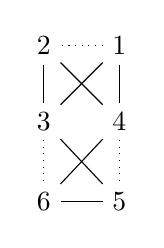
\begin{tikzpicture}
            \node (v0) at (0.38, 2.22) {1};
            \node (v1) at (-0.58, 2.22) {2};
            \node (v2) at (-0.58, 1.26) {3};
            \node (v3) at (0.38, 1.26) {4};
            \node (v4) at (0.38, 0.24) {5};
            \node (v5) at (-0.58, 0.24) {6};
            \draw[dotted] (v0) -- (v1);
            \draw (v0) -- (v3);
            \draw (v0) -- (v2);
            \draw (v1) -- (v2);
            \draw[dotted] (v2) -- (v5);
            \draw (v2) -- (v4);
            \draw[dotted] (v3) -- (v4);
            \draw (v3) -- (v5);
            \draw (v3) -- (v1);
            \draw (v4) -- (v5);
        \end{tikzpicture}
        \end{minipage}
        \caption{Gráfica $G_{2}$ con ciclo $= 2$}
        \label{figura:G2}
     \end{subfigure}
      \caption{Ejemplos de gráficas de tipo $\DynD_{n}$}
      \label{figura:dosEjemplos}
\end{figure}

Descomponemos en su componentes biconexas:
\begin{figure}[H]
     \begin{subfigure}[b]{0.3\textwidth}
     \begin{minipage}{7cm}
        \centering% El subgrafo está centrado
         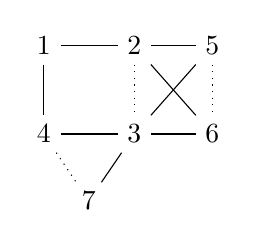
\begin{tikzpicture}
            \node (v0) at (-1.27, 0.36) {1};
            \node (v1) at (-0.12, 0.36) {2};
            \node (v2) at (-0.12, -0.76) {3};
            \node (v3) at (-1.27, -0.76) {4};
            \node (v4) at (0.87, 0.36) {5};
            \node (v5) at (0.87, -0.76) {6};
            \node (v6) at (-0.7, -1.61) {7};
            \draw (v0) -- (v1);
            \draw (v0) -- (v3);
            \draw[dotted] (v1) -- (v2);
            \draw (v1) -- (v4);
            \draw (v1) -- (v5);
            \draw (v2) -- (v3);
            \draw (v2) -- (v5);
            \draw (v2) -- (v4);
            \draw (v2) -- (v6);
            \draw[dotted] (v3) -- (v6);
            \draw[dotted] (v4) -- (v5);
         \end{tikzpicture}
        \end{minipage}
        \caption{$G_{1,1}$}
         \label{figura:G11}
     \end{subfigure}
     \begin{subfigure}[b]{0.3\textwidth}
        \begin{minipage}{7cm}
        \centering% El subgrafo está centrado
         \begin{tikzpicture}
            \node (v6) at (-0.7, -1.61) {7};
            \node (v7) at (-0.39, -2.6) {8};
            \draw (v6) -- (v7);
            \draw (v8) -- (v4);
         \end{tikzpicture}
        \end{minipage}
        \caption{$G_{1,2}$}
        \label{figura:G12}
     \end{subfigure}
     \begin{subfigure}[b]{0.3\textwidth}
        \begin{minipage}{7cm}
        \centering% El subgrafo está centrado
         \begin{tikzpicture}
            \node (v4) at (0.87, 0.36) {5};
            \node (v8) at (0.87, 1.22) {9};
            \node (v9) at (2.12, 0.36) {10};
            \draw[dotted] (v8) -- (v9);
            \draw (v4) -- (v9);
            \draw (v4) -- (v8);
         \end{tikzpicture}
        \end{minipage}
        \caption{$G_{1,3}$}
        \label{figura:G13}
     \end{subfigure}
     \hfill
      \caption{Descomposición de $G_{1}$ en sus componentes biconexas}
      \label{fig:three graphs}
\end{figure}

Arboles generados de el recorrido en profundidad de la componente biconexa que no es de tipo $\DynA_{n}$ de las gráficas:
\begin{figure}[H]
\centering
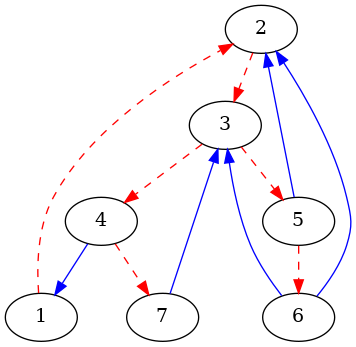
\includegraphics[width=6cm]{Figuras/G3.png}
\caption{Árbol generado en el recorrido primero en profundidad en $G_{1, 1}$}
\label{figura:recorridoG1}
\end{figure}

\begin{figure}[H]
\centering
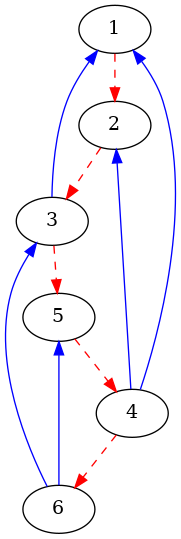
\includegraphics[width=3cm]{Figuras/G4.png}
\caption{Árbol generado en el recorrido primero en profundidad en $G_{2}$}
\label{figura:recorridoG2}
\end{figure}

Calculamos los lowpt1 y lowpt2 de cada gráfica:
\begin{table}[H]
\begin{center}
\begin{tabular}{lll}
\toprule
vertice & lowpt1 & lowpt2 \\
\midrule
      1 &      1 &      1 \\
      2 &      1 &      2 \\
      3 &      1 &      2 \\
      4 &      1 &      3 \\
      5 &      2 &      3 \\
      6 &      2 &      3 \\
      7 &      3 &      5 \\
\bottomrule
\end{tabular}
\caption{Cálculos de lowpt1 y lowpt2 en $G_{1,1}$}
\end{center}
\end{table}

\begin{table}[H]
\begin{center}
\begin{tabular}{lll}
\toprule
vertice & lowpt1 & lowpt2 \\
\midrule
      1 &      1 &      1 \\
      2 &      1 &      2 \\
      3 &      1 &      2 \\
      4 &      1 &      2 \\
      5 &      1 &      2 \\
      6 &      3 &      4 \\
\bottomrule
\end{tabular}
\caption{Cálculos de lowpt1 y lowpt2 en $G_{2}$}
\end{center}
\end{table}

El ordenamiento de $\phi$ en $G_{1, 1}$ da el siguiente resultado:
\begin{center}
1: [2],\\
2: [3],\\
3: [4, 5],\\
4: [1, 7],\\
5: [6, 2],\\
6: [2, 3],\\
7: [3]
\end{center}

Los caminos generados de $G_{1, 1}$ son:
\begin{tabular}[t]{ll}
1: $1 \rightarrow 2 \rightarrow 3 \rightarrow 4 \hookrightarrow 1$ & 2: $4 \rightarrow 7 \hookrightarrow 3$ \\
3: $3 \rightarrow 5 \rightarrow 6 \hookrightarrow 2$ & 4: $6 \hookrightarrow 3$\\
5: $5 \hookrightarrow 2$ & \\
\end{tabular}\\

Solo hay pares de separación de tipo 1 en $G_{1, 1}$ los cuales son $(3, 4), (1, 3), (2, 3)$.

El ordenamiento de $\phi$ en $G_{2}$ da el siguiente resultado:
\begin{center}
1: [2],\\ 
2: [3],\\ 
3: [5, 1],\\ 
4: [1, 2, 6],\\ 
5: [4],\\ 
6: [3, 5]
\end{center}

Los caminos generados de $G_{2}$ son:
\begin{tabular}[t]{ll}
1: $1 \rightarrow 2 \rightarrow 3 \rightarrow 5 \rightarrow 4 \hookrightarrow 1$ & 2: $4 \hookrightarrow 2$ \\
3: $4 \rightarrow 6 \hookrightarrow 3$ & 4: $6 \hookrightarrow 5$\\
5: $3 \hookrightarrow 1$ & \\
\end{tabular}\\

Solo hay un par de separación de tipo 2 en $G_{2}$ el cual es $(3, 4)$.

\begin{figure}[H]
     \begin{subfigure}[b]{0.3\textwidth}
        \begin{minipage}{6cm}
        \centering% El subgrafo está centrado
        \begin{tikzpicture}[scale=.4]
        \GraphInit[vstyle=Normal]
        %
        \tikzset{VertexStyle/.append style={minimum size=1pt, inner sep=1pt}}
        \Vertex[L=\hbox{$3$},x=4.4318cm,y=0.0cm]{v0}
        \Vertex[L=\hbox{$4$},x=0.0cm,y=2.9366cm]{v1}
        \Vertex[L=\hbox{$7$},x=5.0cm,y=5.0cm]{v2}
        %
        \Edge[](v0)(v2)
        \Edge[](v1)(v2)
        \tikzstyle{EdgeStyle}=[color=red]
        \tikzset{LabelStyle/.style = {fill=white, scale=.6}}
        \Edge[label=$A$](v0)(v1)
        %
        \end{tikzpicture}
        \end{minipage}
        \caption{}
         \label{fig:f1}
     \end{subfigure}
     \begin{subfigure}[b]{0.3\textwidth}
        \begin{minipage}{6cm}
        \centering% El subgrafo está centrado
        \begin{tikzpicture}[scale=.4]
        \GraphInit[vstyle=Normal]
        %
        \tikzset{VertexStyle/.append style={minimum size=1pt, inner sep=1pt}}
        \Vertex[L=\hbox{$3$},x=0.0cm,y=0.0cm]{v0}
        \Vertex[L=\hbox{$4$},x=5.0cm,y=5.0cm]{v1}
        %
        \Edge[](v0)(v1)
        \tikzstyle{EdgeStyle}=[color=red]
        \tikzset{LabelStyle/.style = {fill=white, scale=.6}}
        \Edge[label=$A$, style={bend left}](v0)(v1)
        \Edge[label=$B$, style={bend right}](v0)(v1)
        %
        \end{tikzpicture}
        \end{minipage}
        \caption{}
         \label{fig:f1}
     \end{subfigure}
     \begin{subfigure}[b]{0.3\textwidth}
        \begin{minipage}{6cm}
        \centering% El subgrafo está centrado
        \begin{tikzpicture}[scale=.4]
        \GraphInit[vstyle=Normal]
        %
        \tikzset{VertexStyle/.append style={minimum size=1pt, inner sep=1pt}}
        \Vertex[L=\hbox{$1$},x=0.0cm,y=2.3583cm]{v0}
        \Vertex[L=\hbox{$3$},x=5.0cm,y=0.0cm]{v1}
        \Vertex[L=\hbox{$4$},x=4.8519cm,y=5.0cm]{v2}
        %
        \Edge[](v0)(v2)
        %
        \tikzstyle{EdgeStyle}=[color=red]
        \tikzset{LabelStyle/.style = {fill=white, scale=.6}}
        \Edge[label=$C$](v0)(v1)
        \Edge[label=$B$](v1)(v2)
        %
        \end{tikzpicture}
        \end{minipage}
        \caption{}
         \label{fig:f1}
     \end{subfigure}
     \begin{subfigure}[b]{0.3\textwidth}
        \begin{minipage}{6cm}
        \centering% El subgrafo está centrado
        \begin{tikzpicture}[scale=.4]
        \GraphInit[vstyle=Normal]
        %
        \tikzset{VertexStyle/.append style={minimum size=1pt, inner sep=1pt}}
        \Vertex[L=\hbox{$2$},x=2.2651cm,y=0.0cm]{v0}
        \Vertex[L=\hbox{$3$},x=0.0cm,y=2.6956cm]{v1}
        \Vertex[L=\hbox{$5$},x=2.7348cm,y=5.0cm]{v2}
        \Vertex[L=\hbox{$6$},x=5.0cm,y=2.3047cm]{v3}
        %
        \Edge[](v0)(v2)
        \Edge[](v0)(v3)
        \Edge[](v1)(v2)
        \Edge[](v1)(v3)
        \Edge[](v2)(v3)
        \tikzstyle{EdgeStyle}=[color=red]
        \tikzset{LabelStyle/.style = {fill=white, scale=.6}}
        \Edge[label=$D$](v0)(v1)
        %
        \end{tikzpicture}
        \end{minipage}
        \caption{}
         \label{fig:f1}
     \end{subfigure}
     \begin{subfigure}[b]{0.3\textwidth}
        \begin{minipage}{6cm}
        \centering% El subgrafo está centrado
        \begin{tikzpicture}[scale=.4]
        \GraphInit[vstyle=Normal]
        %
        \tikzset{VertexStyle/.append style={minimum size=1pt, inner sep=1pt}}
        \Vertex[L=\hbox{$2$},x=0.0cm,y=5.0cm]{v0}
        \Vertex[L=\hbox{$3$},x=5.0cm,y=0.0cm]{v1}
        %
        \Edge[](v0)(v1)
        \tikzstyle{EdgeStyle}=[color=red]
        \tikzset{LabelStyle/.style = {fill=white, scale=.6}}
        \Edge[label=$D$, style={bend left}](v0)(v1)
        \Edge[label=$E$, style={bend right}](v0)(v1)
        %
        \end{tikzpicture}
        \end{minipage}
        \caption{}
         \label{fig:f1}
     \end{subfigure}
     \begin{subfigure}[b]{0.3\textwidth}
        \begin{minipage}{6cm}
        \centering% El subgrafo está centrado
        \begin{tikzpicture}[scale=.4]
        \GraphInit[vstyle=Normal]
        %
        \tikzset{VertexStyle/.append style={minimum size=1pt, inner sep=1pt}}
        \Vertex[L=\hbox{$1$},x=4.1519cm,y=0.0cm]{v0}
        \Vertex[L=\hbox{$2$},x=0.0cm,y=3.1432cm]{v1}
        \Vertex[L=\hbox{$3$},x=5.0cm,y=5.0cm]{v2}
        %
        \Edge[](v0)(v1)
        \tikzstyle{EdgeStyle}=[color=red]
        \tikzset{LabelStyle/.style = {fill=white, scale=.6}}
        \Edge[label=$C$](v0)(v2)
        \Edge[label=$E$](v1)(v2)
        %
        \end{tikzpicture}
        \end{minipage}
        \caption{}
         \label{fig:f1}
     \end{subfigure}
     \caption{Componentes de separación de $G_{1, 1}$}
     \label{figura:componentesTriconexas}
\end{figure}

En el caso de $G_{2}$ los componentes de separación son iguales a las componentes triconexas finales.

Las componentes triconexas finales de las bigráficas:
\begin{figure}[H]
     \begin{subfigure}[b]{0.5\textwidth}
        \begin{minipage}{7cm}
        \centering% El subgrafo está centrado
        \begin{tikzpicture}[scale=.4]
        \GraphInit[vstyle=Normal]
        %
        \tikzset{VertexStyle/.append style={minimum size=1pt, inner sep=1pt}}
        \Vertex[L=\hbox{$3$},x=0.0cm,y=5.0cm]{v0}
        \Vertex[L=\hbox{$4$},x=5.0cm,y=3.5243cm]{v1}
        \Vertex[L=\hbox{$7$},x=1.3175cm,y=0.0cm]{v2}
        %
        \Edge[](v0)(v2)
        \Edge[](v1)(v2)
        \tikzstyle{EdgeStyle}=[color=red]
        \tikzset{LabelStyle/.style = {fill=white, scale=.6}}
        \Edge[label=$A$](v1)(v0)
        %
        \end{tikzpicture}
        \end{minipage}
        \caption{}
         \label{fig:f1}
     \end{subfigure}
     \begin{subfigure}[b]{0.5\textwidth}
        \begin{minipage}{7cm}
        \centering% El subgrafo está centrado
        \begin{tikzpicture}[scale=.4]
        \GraphInit[vstyle=Normal]
        %
        \tikzset{VertexStyle/.append style={minimum size=1pt, inner sep=1pt}}
        \Vertex[L=\hbox{$3$},x=5.0cm,y=0.0cm]{v0}
        \Vertex[L=\hbox{$4$},x=0.0cm,y=5.0cm]{v1}
        %
        \Edge[](v0)(v1)
        \tikzstyle{EdgeStyle}=[color=red]
        \tikzset{LabelStyle/.style = {fill=white, scale=.6}}
        \Edge[label=$A$, style={bend left}](v0)(v1)
        \Edge[label=$B$, style={bend right}](v0)(v1)
        %
        \end{tikzpicture}
        \end{minipage}
        \caption{}
         \label{fig:f1}
     \end{subfigure}
     \begin{subfigure}[b]{0.3\textwidth}
        \begin{minipage}{7cm}
        \centering% El subgrafo está centrado
        \begin{tikzpicture}[scale=.4]
        \GraphInit[vstyle=Normal]
        %
        \tikzset{VertexStyle/.append style={minimum size=1pt, inner sep=1pt}}
        \Vertex[L=\hbox{$1$},x=5.0cm,y=1.2919cm]{v0}
        \Vertex[L=\hbox{$2$},x=1.4292cm,y=0.0cm]{v1}
        \Vertex[L=\hbox{$3$},x=0.0cm,y=3.5377cm]{v2}
        \Vertex[L=\hbox{$4$},x=3.6225cm,y=5.0cm]{v3}
        %
        \Edge[](v0)(v1)
        \Edge[](v0)(v3)
        \tikzstyle{EdgeStyle}=[color=red]
        \tikzset{LabelStyle/.style = {fill=white, scale=.6}}
        \Edge[label=$E$](v1)(v2)
        \Edge[label=$B$](v2)(v3)
        %
        \end{tikzpicture}
        \end{minipage}
        \caption{}
         \label{fig:f1}
     \end{subfigure}
     \begin{subfigure}[b]{0.3\textwidth}
        \begin{minipage}{7cm}
        \centering% El subgrafo está centrado
        \begin{tikzpicture}[scale=.4]
        \GraphInit[vstyle=Normal]
        %
        \tikzset{VertexStyle/.append style={minimum size=1pt, inner sep=1pt}}
        \Vertex[L=\hbox{$2$},x=5.0cm,y=4.0504cm]{v0}
        \Vertex[L=\hbox{$3$},x=0.1743cm,y=5.0cm]{v1}
        \Vertex[L=\hbox{$5$},x=4.8257cm,y=0.0cm]{v2}
        \Vertex[L=\hbox{$6$},x=0.0cm,y=0.9496cm]{v3}
        %
        \Edge[](v0)(v2)
        \Edge[](v0)(v3)
        \Edge[](v1)(v2)
        \Edge[](v1)(v3)
        \Edge[](v2)(v3)
        \tikzstyle{EdgeStyle}=[color=red]
        \tikzset{LabelStyle/.style = {fill=white, scale=.6}}
        \Edge[label=$D$](v0)(v1)
        %
        \end{tikzpicture}
        \end{minipage}
        \caption{}
         \label{fig:f1}
     \end{subfigure}
     \begin{subfigure}[b]{0.3\textwidth}
        \begin{minipage}{7cm}
        \centering% El subgrafo está centrado
        \begin{tikzpicture}[scale=.4]
        \GraphInit[vstyle=Normal]
        %
        \tikzset{VertexStyle/.append style={minimum size=1pt, inner sep=1pt}}
        \Vertex[L=\hbox{$2$},x=5.0cm,y=0.0cm]{v0}
        \Vertex[L=\hbox{$3$},x=0.0cm,y=5.0cm]{v1}
        %
        \Edge[](v0)(v1)
        \tikzstyle{EdgeStyle}=[color=red]
        \tikzset{LabelStyle/.style = {fill=white, scale=.6}}
        \Edge[label=$D$, style={bend left}](v0)(v1)
        \Edge[label=$E$, style={bend right}](v0)(v1)
        %
        \end{tikzpicture}
        \end{minipage}
        \caption{}
         \label{fig:f1}
     \end{subfigure}
     \caption{Componentes triconexas de $G_{1,1}$}
     \label{figura:componentesTriconexas}
\end{figure}

\begin{figure}[H]
    \begin{subfigure}[b]{0.5\textwidth}
        \begin{minipage}{7cm}
        \centering% El subgrafo está centrado
        \begin{tikzpicture}[scale=.4]
        \GraphInit[vstyle=Normal]
        %
        \tikzset{VertexStyle/.append style={minimum size=1pt, inner sep=1pt}}
        \Vertex[L=\hbox{$3$},x=2.7617cm,y=5.0cm]{v0}
        \Vertex[L=\hbox{$4$},x=5.0cm,y=2.3416cm]{v1}
        \Vertex[L=\hbox{$5$},x=0.0cm,y=2.8439cm]{v2}
        \Vertex[L=\hbox{$6$},x=2.4111cm,y=0.0cm]{v3}
        %
        \Edge[](v2)(v3)
        \Edge[](v0)(v2)
        \Edge[](v0)(v3)
        \Edge[](v1)(v2)
        \Edge[](v1)(v3)
        \tikzstyle{EdgeStyle}=[color=red]
        \tikzset{LabelStyle/.style = {fill=white, scale=.6}}
        \Edge[label=$A$](v0)(v1)
        %
        \end{tikzpicture}
        \end{minipage}
        \caption{}
         \label{fig:f1}
     \end{subfigure}
     \begin{subfigure}[b]{0.5\textwidth}
        \begin{minipage}{7cm}
        \centering% El subgrafo está centrado
        \begin{tikzpicture}[scale=.4]
        \GraphInit[vstyle=Normal]
        %
        \tikzset{VertexStyle/.append style={minimum size=1pt, inner sep=1pt}}
        \Vertex[L=\hbox{$1$},x=4.7286cm,y=5.0cm]{v0}
        \Vertex[L=\hbox{$2$},x=5.0cm,y=0.1367cm]{v1}
        \Vertex[L=\hbox{$3$},x=0.0cm,y=4.8796cm]{v2}
        \Vertex[L=\hbox{$4$},x=0.3559cm,y=0.0cm]{v3}
        %
        \Edge[](v0)(v1)
        \Edge[](v0)(v2)
        \Edge[](v0)(v3)
        \Edge[](v1)(v2)
        \Edge[](v1)(v3)
        \tikzstyle{EdgeStyle}=[color=red]
        \tikzset{LabelStyle/.style = {fill=white, scale=.6}}
        \Edge[label=$A$](v2)(v3)
        %
        \end{tikzpicture}
        \end{minipage}
        \caption{}
         \label{fig:f1}
     \end{subfigure}
     \caption{Componentes triconexas de $G_{2}$}
     \label{figura:componentesTriconexas1}
\end{figure}

Obtenemos ahora la bigráfica original y aplicamos el criterio para decidir si la arista virtual es solida o punteada.
\begin{figure}[H]
     \begin{subfigure}[b]{0.5\textwidth}
        \begin{minipage}{7cm}
        \centering% El subgrafo está centrado
        \begin{tikzpicture}[scale=.6]
        \GraphInit[vstyle=Normal]
        %
        \tikzset{VertexStyle/.append style={minimum size=1pt, inner sep=1pt}}
        \Vertex[L=\hbox{$2$},x=4.01cm,y=2.517cm]{v1}
        \Vertex[L=\hbox{$3$},x=1.7633cm,y=2.517cm]{v2}
        \Vertex[L=\hbox{$5$},x=1.7633cm,y=4.5228cm]{v4}
        \Vertex[L=\hbox{$6$},x=4.01cm,y=4.5228cm]{v5}
        %
        \Edge[](v1)(v4)
        \Edge[](v1)(v5)
        \Edge[](v2)(v4)
        \Edge[](v2)(v5)
        \Edge[style=dashed](v4)(v5)
        \Edge[style=dashed](v1)(v2)
        %
        \end{tikzpicture}
        \end{minipage}
        \caption{}
         \label{fig:f1}
     \end{subfigure}
     \begin{subfigure}[b]{0.5\textwidth}
        \begin{minipage}{7cm}
        \centering% El subgrafo está centrado
        \begin{tikzpicture}[scale=.6]
        \GraphInit[vstyle=Normal]
        %
        \tikzset{VertexStyle/.append style={minimum size=1pt, inner sep=1pt}}
        \Vertex[L=\hbox{$2$},x=4.31cm,y=3.2064cm]{v1}
        \Vertex[L=\hbox{$3$},x=1.7633cm,y=2.517cm]{v2}
        %
        \Edge[](v1)(v2)
        %
        \end{tikzpicture}
        \end{minipage}
        \caption{}
         \label{fig:f1}
     \end{subfigure}
     \begin{subfigure}[b]{0.3\textwidth}
        \begin{minipage}{7cm}
        \centering% El subgrafo está centrado
        \begin{tikzpicture}[scale=.6]
        \GraphInit[vstyle=Normal]
        %
        \tikzset{VertexStyle/.append style={minimum size=1pt, inner sep=1pt}}
        \Vertex[L=\hbox{$3$},x=1.3633cm,y=2.517cm]{v2}
        \Vertex[L=\hbox{$4$},x=2.3604cm,y=0.0cm]{v3}
        \Vertex[L=\hbox{$7$},x=0.0cm,y=0.0cm]{v6}
        %
        \Edge[](v2)(v3)
        \Edge[](v2)(v6)
        \Edge[style=dashed](v3)(v6)
        %
        \end{tikzpicture}
        \end{minipage}
        \caption{}
         \label{fig:f1}
     \end{subfigure}
     \begin{subfigure}[b]{0.3\textwidth}
        \begin{minipage}{7cm}
        \centering% El subgrafo está centrado
        \begin{tikzpicture}[scale=.6]
        \GraphInit[vstyle=Normal]
        %
        \tikzset{VertexStyle/.append style={minimum size=1pt, inner sep=1pt}}
        \Vertex[L=\hbox{$3$},x=1.7633cm,y=2.317cm]{v2}
        \Vertex[L=\hbox{$4$},x=2.3604cm,y=0.0cm]{v3}
        %
        \Edge[](v2)(v3)
        %
        \end{tikzpicture}
        \end{minipage}
        \caption{}
         \label{fig:f1}
     \end{subfigure}
     \begin{subfigure}[b]{0.3\textwidth}
        \begin{minipage}{7cm}
        \centering% El subgrafo está centrado
        \begin{tikzpicture}[scale=.6]
        \GraphInit[vstyle=Normal]
        %
        \tikzset{VertexStyle/.append style={minimum size=1pt, inner sep=1pt}}
        \Vertex[L=\hbox{$1$},x=5.0cm,y=0.0cm]{v0}
        \Vertex[L=\hbox{$2$},x=5.0cm,y=2.517cm]{v1}
        \Vertex[L=\hbox{$3$},x=2.3604cm,y=2.517cm]{v2}
        \Vertex[L=\hbox{$4$},x=2.3604cm,y=0.0cm]{v3}
        %
        \Edge[](v0)(v1)
        \Edge[](v0)(v3)
        \Edge[](v1)(v2)
        \Edge[style=dashed](v2)(v3)
        %
        \end{tikzpicture}
        \end{minipage}
        \caption{}
         \label{fig:f1}
     \end{subfigure}
     \caption{Componentes triconexas de $G_{1,1}$}
     \label{figura:componentesTriconexas}
\end{figure}

De el capitulo 2 sabemos que estas gráficas excepto (e) son $\DynA$-bloques.

\begin{figure}[H]
    \begin{subfigure}[b]{0.5\textwidth}
        \begin{minipage}{7cm}
        \centering% El subgrafo está centrado
        \begin{tikzpicture}[scale=.6]
        \GraphInit[vstyle=Normal]
        %
        \tikzset{VertexStyle/.append style={minimum size=1pt, inner sep=1pt}}
        \Vertex[L=\hbox{$3$},x=2.8524cm,y=2.0745cm]{v2}
        \Vertex[L=\hbox{$4$},x=0.3702cm,y=2.0745cm]{v3}
        \Vertex[L=\hbox{$5$},x=2.8524cm,y=4.8114cm]{v4}
        \Vertex[L=\hbox{$6$},x=0.3702cm,y=4.8114cm]{v5}
        %
        \Edge[](v2)(v3)
        \Edge[](v2)(v4)
        \Edge[style=dashed](v2)(v5)
        \Edge[](v4)(v5)
        \Edge[style=dashed](v4)(v3)
        \Edge[](v3)(v5)
        \Edge[](v2)(v3)
        %
        \end{tikzpicture}
        \end{minipage}
        \caption{}
         \label{fig:f1}
     \end{subfigure}
     \begin{subfigure}[b]{0.5\textwidth}
        \begin{minipage}{7cm}
        \centering% El subgrafo está centrado
        \begin{tikzpicture}[scale=.6]
        \GraphInit[vstyle=Normal]
        %
        \tikzset{VertexStyle/.append style={minimum size=1pt, inner sep=1pt}}
        \Vertex[L=\hbox{$1$},x=4.4008cm,y=0.0cm]{v0}
        \Vertex[L=\hbox{$2$},x=4.4008cm,y=2.7015cm]{v1}
        \Vertex[L=\hbox{$3$},x=1.8549cm,y=2.7015cm]{v2}
        \Vertex[L=\hbox{$4$},x=1.8549cm,y=0.0cm]{v3}
        %
        \Edge[style=dashed](v0)(v1)
        \Edge[](v0)(v2)
        \Edge[](v1)(v2)
        \Edge[](v3)(v1)
        \Edge[](v3)(v0)
        \Edge[style=dashed](v2)(v3)
        %
        \end{tikzpicture}
        \end{minipage}
        \caption{}
         \label{fig:f1}
     \end{subfigure}
     \caption{Componentes triconexas de $G_{2}$}
     \label{figura:componentesTriconexas1}
\end{figure}





